\documentclass[conference]{IEEEtran}
\IEEEoverridecommandlockouts

\usepackage{cite}
\usepackage{amsmath,amssymb,amsfonts}
\usepackage{algorithmic}
\usepackage{graphicx}
\usepackage{textcomp}
\usepackage{xcolor}
\def\BibTeX{{\rm B\kern-.05em{\sc i\kern-.025em b}\kern-.08em
    T\kern-.1667em\lower.7ex\hbox{E}\kern-.125emX}}
\begin{document}

\title{Fake News Detection using Machine Learning}



\author{

\IEEEauthorblockN{1\textsuperscript{st} Joy Barai}
\IEEEauthorblockA{\textit{dept. of CSE } \\
\textit{East West University}\\
Dhaka, Bangladesh \\
2018-1-60-011}
\and

\IEEEauthorblockN{2\textsuperscript{nd} Maleha Israt Chowdhury}
\IEEEauthorblockA{\textit{dept. of CSE } \\
\textit{East West University}\\
Dhaka, Bangladesh \\
2018-1-60-015}
\and

\IEEEauthorblockN{3\textsuperscript{rd} Kamarum Monira Mow}
\IEEEauthorblockA{\textit{dept. of CSE } \\
\textit{East West University}\\
Dhaka, Bangladesh \\
2018-1-60-016}
\and



\IEEEauthorblockN{4\textsuperscript{th} Tashfia Choudhury}
\IEEEauthorblockA{\textit{dept. of CSE } \\
\textit{East West University}\\
Dhaka, Bangladesh \\
2018-1-60-045}

}

\maketitle

\begin{abstract}

Nowadays internet is important and available on the hands of common people. There are too many news portals and social media where news can be broadcast easily. Obviously some people want to gain the advantages from this. They use click bate for their own profits. Sometimes these are more serious , when someone try to spread rumor through those platforms.Its tough to control cause these sites do not verify these posts and people can believe anything which is well represented.As its not easy to detect fake news for everyone so by using machine learning classifier this problem is solvable.

\end{abstract}

\vspace{12pt}


\begin{IEEEkeywords}
ake news; Machinea learning; Natural Language Processing ; Multinomial; Logistic Regression; Passive Agressive
\end{IEEEkeywords}

\section{Introduction}
Fake news detection refers to the news that is full of alteration and deception of information and spreads without having any authenticated source that is needed to be detected. This misleading information costs certain services of a nation or its citizens. Many ways have been used to detect such news to avoid spreading and misleading. This could not be done as it is still dependent on human manual detection. Moreover, Social media has become a fast-growing thing. It has become quite easy to spread any fake news or article rapidly. Now a day’s such fake news is created to fulfill some agenda. So many news and articles keep circulated on every social media platform that it has become quite impossible to detect which news is real and which is fake. Human evaluation has become challenging to detect authenticity.[1] In such a scenario Machine learning approach to detect fake news and labeled it is the only approach that can reduce this problem.
The purpose of this paper is to create a model that will be able to identify if an article is fake or not based on its words, phrases, source, and titles by applying some supervised machine learning algorithm on an annotated dataset[2]. The model will be tested by using different classifications, on the processed dataset and evaluate the results.

\subsection{Objectives}
The main objective is to detect fake news that is labeled with standard text with a straightforward proposition. Fake news detection is made to stop spreading wrong and deceptive news. A model that can differentiate between real and fake news is needed. This fake news gets more viral on social media sites like Facebook, Twitter, and messaging apps like WhatsApp, Hike, and Viber around the world[3]. The model can distinguish between true and false news and can help to find authentic news or article.


\subsection{Motivation}
Nowadays it’s a major issue to the media and electronic channels that there are many sources and news. As the authority is not taking any steps for those web-based news portals, those portals are growing faster. Here and there, there is so much news those are conflicting sometimes with one another. As being a common people, it is quite hard to find out which is the true news and which one is false. As we know there are concepts like clickbait, it is a trap to attract people with catchy headlines or thumbnails. Newborn news portals are doing these things a lot nowadays. Sometimes the intentions are not so good or innocent at all. Record says that it is about 43 percent  of fake news are for spreading rumor and gathering the self-benefit of the news portal. Sometimes different parties hire private news portals for spreading rumors for their benefit. It is kind of hard to define which news is true. So, it is quite necessary to detect false news as soon as someone reads those. This is the basic reason we are intended to working on this. Projects like this can control emergencies from spreading a rumor and keep those common men in a calm society [4]

\subsection{Existing Work}
It is a global issue nowadays cause a survey from 2016 by BuzzFeed found that 75 percent of American adults are fooled by fake news.[5] The problem of detecting deception is not new to natural language processing (Vargo et al., 2018). Significant application domains include detecting false online advertising, fake consumer reviews, and spam emails (Ott et al., 2011) (Zhang and Guan, 2008). The detection of fake news focuses on uncovering the spread of misleading news articles (Zhou and Zafarani, 2020) (Zhou et al., 2019). Typical detection techniques use either text-based linguistic features (Potthast et al., 2018) or visual features (Gupta et al., 2013). Overall, fake news detection methods fall into two groups: knowledge-based models based on fact-checking news articles using external sources (WuYou et al., 2014), and style-based models, which leverage linguistic features capturing writing style (Rubin and Lukoianova, 2015). Many studies such as (Wang, 2017) (Mitra and Gilbert, 2015) (Shu et al., 2020a) incorporate publicly available datasets, providing a basis for detailed analysis of fake news and detection methods. Recently, deep learning-based latent representation of text has significantly improved fake news classification accuracy (Karimi and Tang, 2019).[6] 
 
In 2021 a four members team worked on exactly this topic from Technische University Berlin. They tested this by checking if automated augmentation of fake news sentences (FALSE statements) will lead to TRUE classifications. This would allow them to bypass the fake news detection mechanisms. Our results show that using the python library TextAttack allows automated changing of classification for 65,15 percent of the sentences. Flair, the only model using word-level embedding (contextual string embeddings), seems less vulnerable to attacks with a Success Rate of 54,77 percent. The other two models using document embeddings show 72,45 percent (BERTweet) and 68,22percent (Roberta). [7]
If we stare at another work from Brawijaya University, they used three data sources with a total data reaching 2,216 with a distribution of 1,055 as valid data and 1,161 as false data. The dataset is then divided into data with a ratio of 80 percent: 20percent for training data and test data sequentially. So that the total training data used is 1772 and 444 test data. [8]

\subsection{Necessity}
As long as this is a global problem, this problem has to be sorted out by researchers. Misinformation is spreading at increasing rates particularly online, and is considered a highly pressing issue by the World Economic Forum. To combat this problem, automatic fact-checking, especially for estimating the veracity of potentially fake news, has been extensively researched. Most of the fact-checking systems are based on evidence-based. It means, they are using external knowledge to determine the claims and that knowledge may be connected with the previous fact-checking assumptions or probability. The system works like they are using a claim to examine the web by searching the API with relevant things. When these things are well tackled by the researchers and finally a fruitful result comes to light, it helps everybody beyond the globe to understand the authenticity of the news.[9] 


\section{Methodology}
As detecting fake news is so much important for the globe, we are working with some different perspectives here. First of all, we need to collect data for pre-processing those with TF/IDF. Then we train those data with different models. 
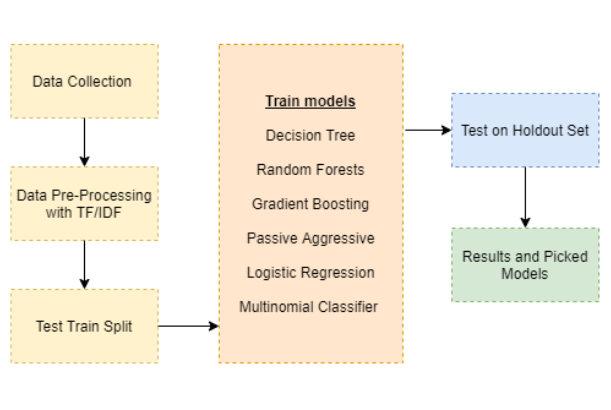
\includegraphics[scale=0.55]{figA.png}
Figure 1: the flowchart we follow for the whole project

\subsection{Multinomial Naïve Bayes}
Multinomial classifier belongs to the Naïve Bayes family. According to this category, the classification is based on Bayes` rule or Bayes` formula. The Bayes Formula is- 
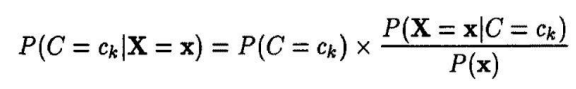
\includegraphics[scale=0.55]{figB.png}
And the Bayes Rules is-
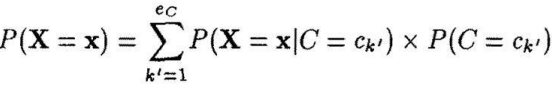
\includegraphics[scale=0.55]{figC.png}
C is a variable that includes all the possible events. In this study, the variable C contains all the documents of the dataset, is a vector random variable of the feature values x = (x1,..,xj ,…,xd). Each document has one vector. P(C is the conditional probability that a document belongs to class ck.
The Naive Bayes Classifier is a classifier that uses these equations to achieve its objective. In terms of the following, a multinomial classifier is an alternative technique.
Assumption:
Single draw on a vector-valued variable X of length d using Nave Bayes.
f uses a d-valued multinomial variable X as a source of data.
Finally, in our investigation, the benefit of the Multinomial classifier is that the document length is reduced. In the model, this is resolved quite naturally. On the other side, this has a drawback. According to the study, a classifier implies independence between several variables.

\subsection{Passive Aggressive}
It’s a classifier that belongs to large-scale learning.  It doesn’t need any learning rate to work proficiently. In this case, it is quite similar to perception too. With some sequence rounds, a binary classification consists. Each round, the algorithm examines a new case and predicts whether the label will be +1 or -1. The error is calculated when the prediction is complete, and the algorithm modifies it to learn more about the weight vector and enhance its performance.
sign(w • x), where x is the instance, is the weight vector. When the margin is positive, sign(wt • xt ) = yt (where y is the label), and the algorithm has given an accurate forecast. The classifier's name is linked to the corresponding updating strategy. The constrained optimization problem for round t and new weight vector Wt+1 is presented in more detail-
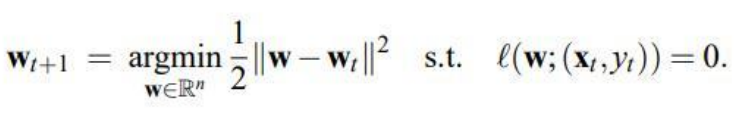
\includegraphics[scale=0.45]{figD.png}
this is weights for PA algorithm
Passive algorithm: Hinger-loss is zero, hence wt+1 = w whenever lt = 0.
The algorithm is aggressive since the loss is positive and wt+1 is compelled to satisfy the condition.
The algorithm is known as Passive-Aggressive because of these two characteristics. It's worth noting that the weight has increased as a result of the aggressive update method.


\subsection{Logistic Regression}
For binary classification issues, logistic regression is the best regression approach. To characterize the data and the connection between one dependent binary variable and one or more independent variables, logistic regression is employed. The goal of logistic regression is to determine the model that best explains the connection between a dependent variable and a set of independent variables.
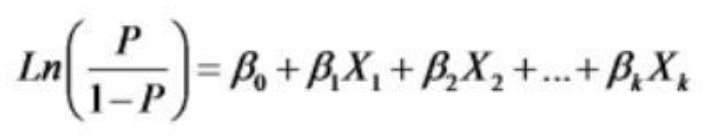
\includegraphics[scale=0.45]{figE.png}
This is the Logistic Function.

The natural log of the changes that the dependent variable is equal to one of the categories is the function. Finally, logistic regression is often used since the logit function is straightforward in terms of interpretation of the findings.

First of all, we collect the dataset from Kaggle and the dataset has total 5 columns in total. Then we just remove all the numbers, special characters, suffixes, and prefixes from those articles. We give priority to those words, those are helping to keep the sentences meaningful. Then we convert the lines to individual vectors and change them to numerical. When we apply multinominal functions to the numerical datasets, it generates some accuracy rate and confusion matrix. Then we apply logistic regression and passive-aggressive, and these things generate another accuracy rate and confusion matrix.


\section{Implementation}
In this section, we will first discuss the dataset, then secondly the necessity of preprocessing to get a clean dataset will be also mentioned, thirdly model development using the dataset and result basis on classification implementation on the dataset.
\subsection{Data Collection}
Data collection is the most important step as most of the effort to detect fake news gets limited because of data. There are many ways to collect data such as fast checking, industry detector, online platform (kaggle, github), and expert journalists[3]. We have used open-source data in this study. The data is combined of both real and fake news articles from different sources. The data set we have used is available in Kaggle[10]. There are two sorts of data set one is a training dataset, another one is test data set. The train data has five features. The first feature contains a unique ID for every article. Then feature names title and author contains the details of title and author of news. Then the body part of the article comes under the text feature. It contains all the information on the news. Lastly, the most important feature on the training data set is the label. The label indicates if an article is reliable or not. If an article is reliable then the label is indicated by 0 and if not the label is 1 indicating the news is fake. The training data contains 20800 number samples. All the features except the label are in the train data set. 

\subsection{Data Pre-Processing}
The data set collected for fake news detection is a raw data set. This data set contains noise such as missing values or special characters, suffix and prefix, commonly used words. Such a dataset needs to be preprocessed. As the performance of any machine learning depends on the input data set. The data needs to be clean for better results. So preprocessing plays an important role.[11] We have followed some steps in our project for preprocessing.

\begin{itemize}
\item \textbf{Natural Language Processing}


Anomalies can be identified by using natural language processing. It separates text articles that are misleading in nature but based on facts. By using the python library natural language toolkit(NLTK) we have made the data preprocessed and clean from redundant words[12]. After the article texts get clean they get converted to numeric data that is a vector feature. Then we used our training algorithm on it. 



\item \textbf{Removed number}


In a particular text, any number does not change the meaning of a sentence. Therefore if it is removed from the article then it will minimize the noise in the data. We have used a python library to keep all alphabet values in the dataset and remove all numerical values. It effectively removes all the numeric values minimizing noise in our dataset.


\item \textbf{Removed punctuation and special characters}


We have only kept the textual data in our project. In this case, we have removed all characters that are special characters or not alphabets. We used the python library for removing all specialized characters[13]. These characters are often used in articles or different news on social media. All these characters do not create any meaning to the sentence so by removing it we didn’t change any meaning of any article or news.[1] After removing special characters we removed punctuation that is not necessary to interpret a meaningful sentence. After removing special characters and punctuation we only kept the word of the text in our data. We made all the text into lowercase and make sure we only have text with English words and no extra symbol is on the dataset.

\vspace{12pt}

\item \textbf{Removed stop words}


Words that are most common or repeated in a list are stop words. After removing numbers, punctuation, and special character the data set only contains words. There are lots of words that are not meaningful and repetitive. So removing such words has made our dataset simpler. It also reduced noise as the only meaningful word is present in the dataset. It also reduced memory as a large portion of a sentence is cut. By using the python library of stop words we have kept only the meaning full word in our data set. 


\item \textbf{Use of stemmer}


There are many words with same meaning, stemming technique removes such word from beginning or end. This method was really useful in our project. This technique helps to distinguish between meaningful and non-meaningful difference of word. We eliminated those words by using python library PorterStemmer and removed more noise from the dataset. Now, the data set is simpler than before and have only words that creates values in sentence.

\end{itemize}



\subsection{Model Development}
TF-IDF is the only model we have used in our project.

\begin{itemize}

\item \textbf{TF-IDF Model}


One of the effective algorithms is TF-IDF in the case of the pre-training vectorization dataset. In the entire corpus occurrence of words is considered by this algorithm. A mathematical formula for calculating TF-IDF is, 



Wt, d = TFt,d log(N/DFt) 



Where, TFt,d is the number of occurrences of t in document d 



 DFt is the number of documents containing the term t. 
N is the total number of documents in the collection of documents
Words that are not much occurred will have a low value of TF-IDF and common words have a high value. We have using TF- IDF vectorization for our dataset. It represented all words into numerical value by making it simpler for the classification to give accurate results[14].



\end{itemize}

\vspace{12pt}


After processing the data set we have implemented three known machine language classificitation such as Multinomial,Logistic Regression and  Passive Aggressive and  got best result out from them .



\subsection{Coding Environment, Language, and tools}

We chose Google Colab as our coding environment for two main reasons. Firstly, to document the process step by step. Secondly, apart from that, we wanted to take advantage of the free GPU in Google Colab. In comparison to our PC, the available GPU helped me train faster. (Of course, we'll note that the resource was depleted after two epochs, but we built a checkpoint to save the model). GPU-powered AWS frameworks, such as AWS Sagemkaer and Google GPU cloud infrastructure, are also beneficial in production for training models and deploying faster. 



Fake news detection is an advanced project where the difference between real and fake news needs to be detected clearly. As python has advanced library features and easily can distinguish between fake and real. So we have chosen Python language for our project.
Since we have used python language we have used python libraries tools for our project to implement our machine learning algorithms and to extract accurate results.


\subsection{Results}

After implementing all the three classification algorithms we have got an accurate result. We prepared a confusion matrix and a table for comparing all three Machine learning algorithms. 



The Confusion Matrix for all the algorithms we have implemented are given below




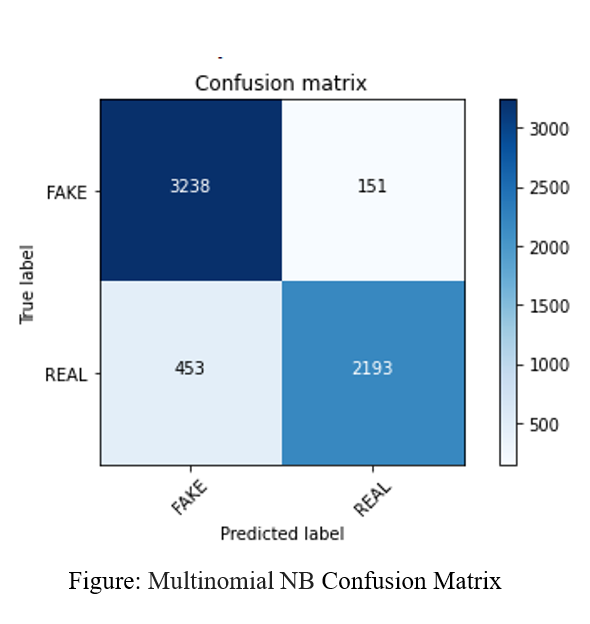
\includegraphics[scale=0.45]{figF.png}
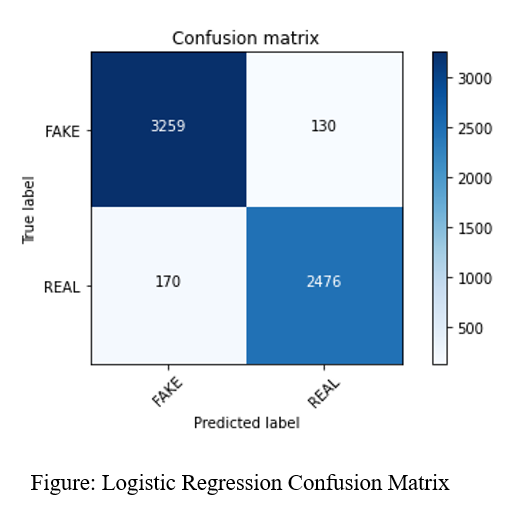
\includegraphics[scale=0.55]{figG.png}
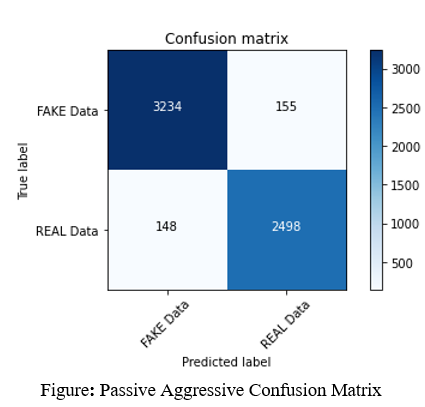
\includegraphics[scale=0.70]{figH.png}


\begin{itemize}
\item \textbf{Table 1}
\begin{table}[ht]
	\centering
	\begin{tabular}{|c|c|c|}
	\hline
	Model & Classifier & Accuracy (percentage) \\
	\hline
	TF-IDF & Multinominal NB & 89.99 \\
	\hline
	TF-IDF & Passive Aggressive NB & 94.98 \\
	\hline
	TF-IDF & Logistic Regression & 95.03 \\
	\hline
	\end{tabular}	
\end{table}
\end{itemize}


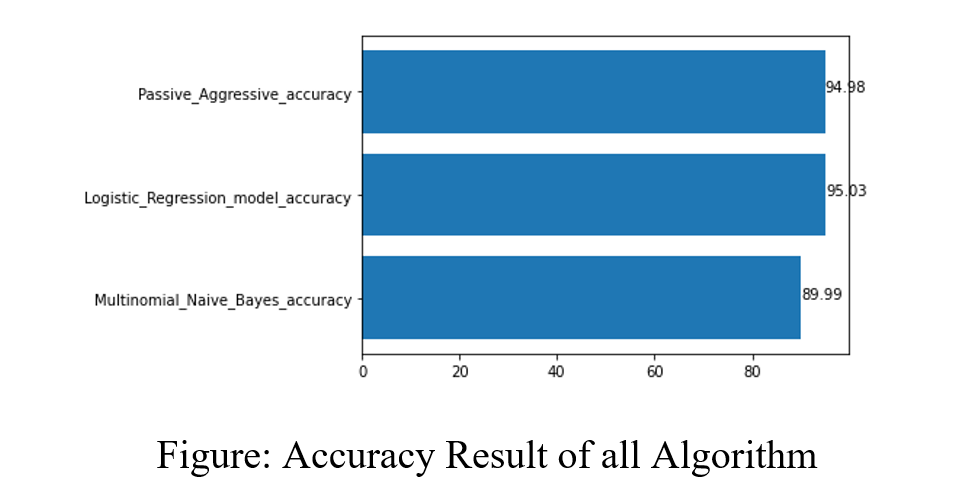
\includegraphics[scale=0.35]{figI.png}

After analyzing all three classifier accuracy rate we can concluded that Logistic Regression Classier has more accuracy to detect fake and real news comparing to other to Classifier


\section{Conclusion}
When the popularity of social media is increasing day by day; straightly it is growing its consumers a lot faster. The fact is more people collect news from social media than the news portals. Even the third-party news portals are out of accountability, so it is quite tough to believe news from easily accessible portals nowadays. [15] As, social media is also a carrier of fake news, that has a serious negative impact on society. In our project, we collected data from an authentic source and pre-processed those bt TF/IDF. Then we test train and split those data as our preference. We used some models to train data like Decision Tree, Random Forest, Gradient Boosting, Passive Aggressive, etc. The algorithms we used were passive-aggressive classifier, multinominal classifier, and logistic regression. Then we just test on the Holdout set and after getting the result we just picked the model which gave us the best result. 


\subsection{Challenges}
During the whole project we faced the main challenge which was dataset. We collect the data set from Kaggle but it is never assured that the dataset is authentic. If the dataset is not authentic then we can not find a perfect result or we cannot verify if our system is working fine or not. 


\subsection{Future Direction}

We worked for our default database which was declared in our system. After working with this process we wanted to work with manual input of data and that was not working fluently. So, there is a big scope to work on if the system can take input from the user and analysis any manually given data. 

\vspace{12pt}
\vspace{12pt}
\vspace{12pt}

\begin{thebibliography}{00}
\bibitem{b1} A. Lakshmanarao, Y. Swathi, and T. Srinivasa Ravi Kiran, “An effecient fake news detection system using machine learning,” Int. J. Innov. Technol. Explor. Eng., vol. 8, no. 10, pp. 3125–3129, 2019, doi: 10.35940/ijitee.J9453.0881019.


\vspace{12pt}
\bibitem{b2} Z. Khanam, B. N. Alwasel, H. Sirafi, and M. Rashid, “Fake News Detection Using Machine Learning Approaches,” IOP Conf. Ser. Mater. Sci. Eng., vol. 1099, no. 1, p. 012040, 2021, doi: 10.1088/1757-899x/1099/1/012040.

\vspace{12pt}
\bibitem{b3} A. Jain and A. Kasbe, Fake News Detection, no. December. 2018


\vspace{12pt}
\bibitem{b4} D. M. J. Lazer et al., “The science of fake news: Addressing fake news requires a multidisciplinary effort,” Science (80-. )., vol. 359, no. 6380, pp. 1094–1096, 2018, doi: 10.1126/science.aao2998.


\vspace{12pt}
\bibitem{b5} H. de Wet and V. Marivate, “Is it Fake? News Disinformation Detection on South African News Websites,” p. 6, 2021, [Online]. Available: http://arxiv.org/abs/2108.02941.


\vspace{12pt}
\bibitem{b6} B. Bhattarai, O.-C. Granmo, and L. Jiao, “Explainable Tsetlin Machine framework for fake news detection with credibility score assessment,” no. 1, p. 11 pages, 2021, [Online]. Available: http://arxiv.org/abs/2105.09114.


\vspace{12pt}
\bibitem{b7} C. Koenders, J. Filla, N. Schneider, and V. Woloszyn, “How Vulnerable Are Automatic Fake News Detection Methods to Adversarial Attacks?,” 2021, [Online]. Available: http://arxiv.org/abs/2107.07970

\vspace{12pt}
\bibitem{b8} A. Awalina, “Indonesia’s Fake News Detection using Transformer Network.”
\vspace{12pt}
\bibitem{b9} C. Hansen, C. Hansen, and L. Chaves Lima, “Automatic Fake News Detection:Are Models Learning to Reason?,” pp. 80–86, 2021, doi: 10.18653/v1/2021.acl-short.12
\vspace{12pt}
\bibitem{b10} Kaggle, “Fake News,” Kaggle,San Francisco; CA; USA, 2018. https://www.kaggle.com/c/fake-news/data.
\vspace{12pt}
\bibitem{b11} Sid, “Improving Fake News Detection with Linguistic Cues Koumouridis Georgios,” no. December, 2019.
\vspace{12pt}
\bibitem{b12} I. Ahmad, M. Yousaf, S. Yousaf, and M. O. Ahmad, “Fake News Detection Using Machine Learning Ensemble Methods,” Proc. - 2020 IEEE Int. Symp. Sustain. Energy, Signal Process. Cyber Secur. iSSSC 2020, vol. 2020, 2020, doi: 10.1155/2020/8885861.
\vspace{12pt}
\bibitem{b13} S. Vijayaraghavan et al., “Fake News Detection with Different Models,” 2020, [Online]. Available: http://arxiv.org/abs/2003.04978.
\vspace{12pt}
\bibitem{b14} J. Ramos, “Using TF-IDF to Determine Word Relevance in Document Queries,” Proc. first Instr. Conf. Mach. Learn., vol. 242, no. 1, pp. 29–48, 2003
\vspace{12pt}
\bibitem{b15} K. Shu, “Fake News Detection on Social Media: A Data Mining Perspective.”


\end{thebibliography}



\vspace{12pt}


\end{document}
